% !Mode:: "TeX:UTF-8" (encoding info for WinEdt)
\section{Codes des diagnostics Suisses sous Elexis}
Intégration de CIM-10 et du code tessinois comme codes des diagnostics pour la consultation. Ce plugin fait partie de la distribution standard de Elexis.
\subsection{CIM-10}
\begin{wrapfigure}{r}{7cm}
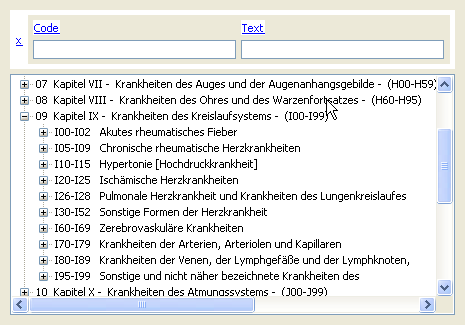
\includegraphics[width=7cm]{images/icd10}
\caption{ICD-10}
\label{fig:icd10}
\end{wrapfigure}

Le plugin lui-même contient par contre que les structures et les données doivent encore être importées. Des plus amples informations vous trouvez sous  \ref{config:icd10} à la page \pageref{config:icd10}.

\medskip

CIM-10 est un code basé sur une structure hiérearchique. Comme vous pouvez constater sous \ref{fig:icd10} cette structure peut être visualisée den forme d'un arbre. Pour ouvrir une branche on peut cliquer sur le petit signe + qui se trouve à gauche à côté du nom.

En Suisse certains assureurs (AI, AM et LAA) attendent qu'on mette sur la facture Tarmed un code CIM_10 comme diagnostic.

\subsection{Code tessinois (TI-Code)}
Le code tessinois est un code de diagnostic très simple qui ne contient qu'une spécification très générale de la maladie. Les assureurs maladie demandent l'introduction du code tessinois comme diagnostic sur la facture Tarmed. Puisque ceci peut porter préjudice au patient car le secrét médical n'est plus garantie par le fait que les médecins transmettent ce code aux fonctionnaires des assurances, beaucoup de patients refusent par écrit que les médecins mettent ce code sur la facture.

L'importation des données n'est pas nécessaire (les données se trouvent déjà dans le plugin). Il y a une version en Allemand, Français et Italien du code tessinois.